\documentclass{../exhibit}

\title{Carousing with Pirates}

%% Font
\usepackage{imfellEnglish}
\usepackage[T1]{fontenc}
\raggedright

\usepackage[LGRgreek]{mathastext}


%% so title is accessable
\makeatletter
\let\thetitle\@title
\let\theabstract\@abstract
\makeatother


\usepackage{background}
\backgroundsetup{
scale=1,
color=white,
opacity=0.2,
angle=0,
contents={%
  \hspace{0 in}\raisebox{0 in}{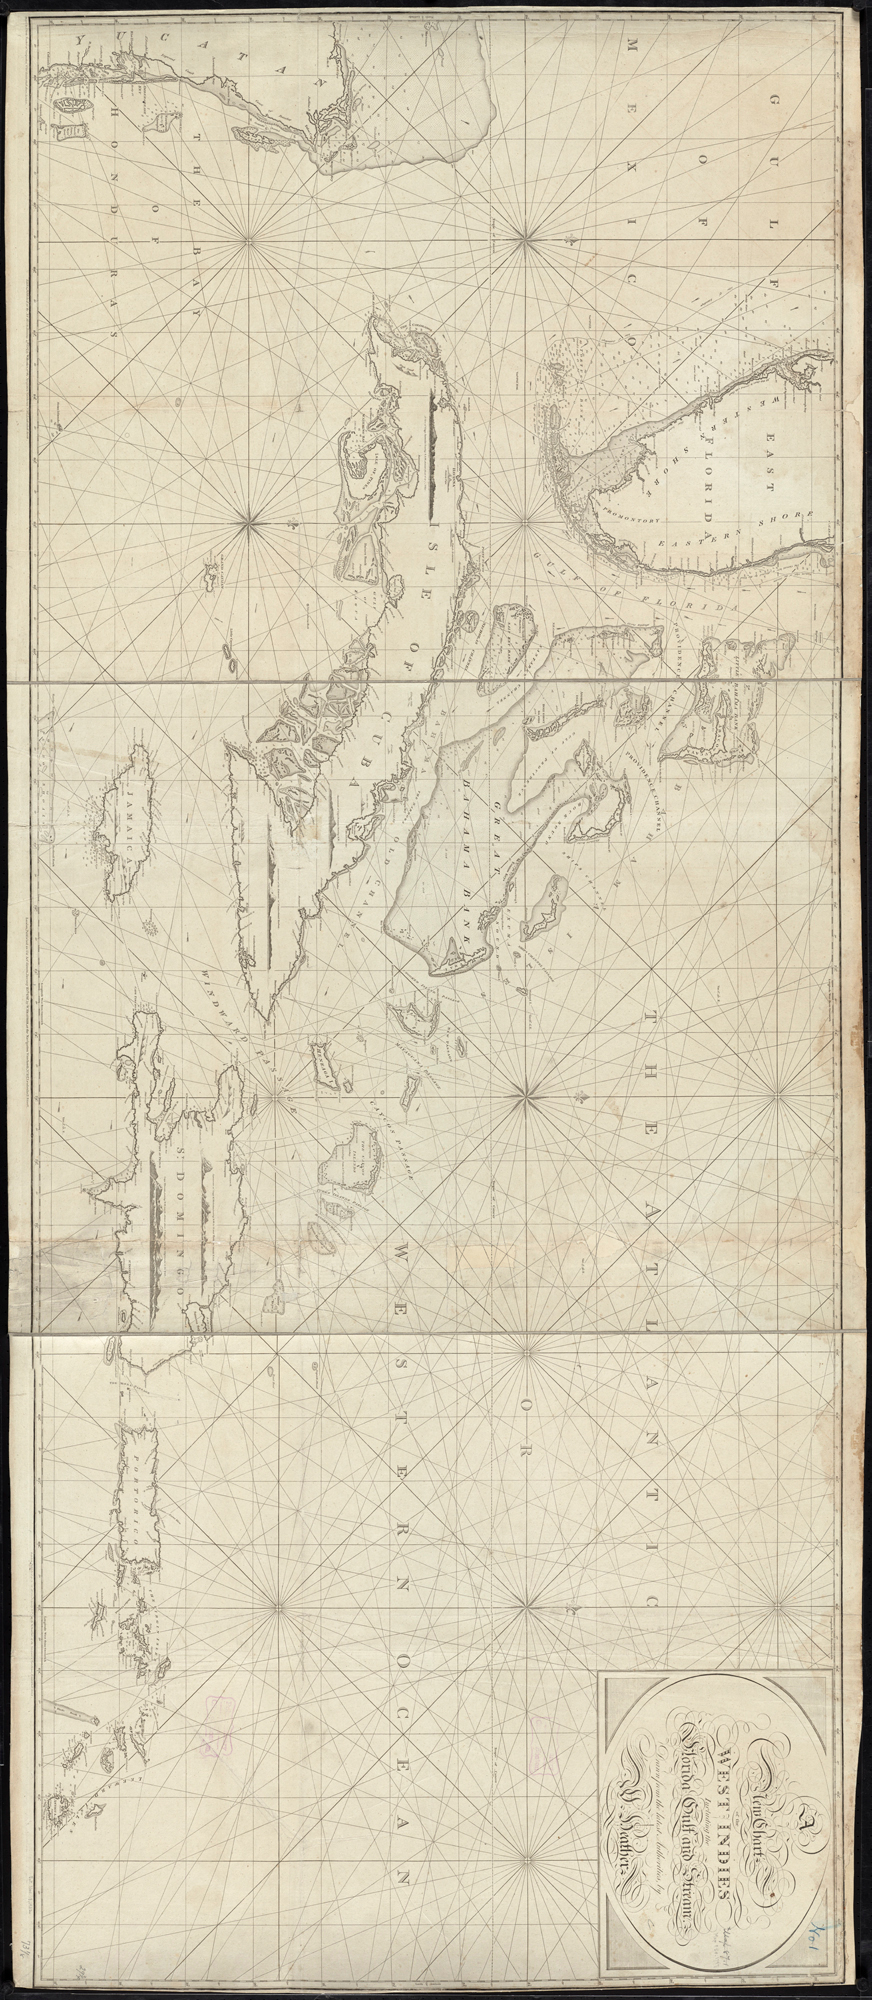
\includegraphics[scale=.5]{mapBackground.jpg}}
  %%https://commons.wikimedia.org/wiki/File:1683_Mortier_Map_of_North_America,_the_West_Indies,_and_the_Atlantic_Ocean_-_Geographicus_-_Atlantique-mortier-1693.jpg
  }%
}


\def\imagetop#1{\vtop{\null\hbox{#1}}}

%% For the context
%% https://tex.stackexchange.com/questions/86150/torn-page-effect/86151#86151
\usepackage{tikz}
\usetikzlibrary{decorations.pathmorphing}
\definecolor{paper}{RGB}{239,227,157}


%% QR code
\usepackage{qrcode}



%% For bold-ish title
\usepackage{shadowtext}



\renewcommand{\maketitle}{ %
  \shadowoffset{.5pt} %% See: https://tex.stackexchange.com/questions/159463/fancy-styled-borders-in-latex
  \shadowcolor{black!50!white}
  \begin{center}
    \resizebox{\textwidth}{!}{\shadowtext{\scshape\thetitle}}
  \end{center}
  
\vspace{1cm}
  
\begin{tabular*}{\textwidth}{c @{\extracolsep{\fill}} c}  
  \imagetop{
\begin{tikzpicture}
        \node[preaction={fill=white,opacity=0},inner sep=.5cm] 
             {
               \begin{minipage}{.45\textwidth}\Huge\directions\end{minipage}
             };
  \end{tikzpicture}}
  &
  \imagetop{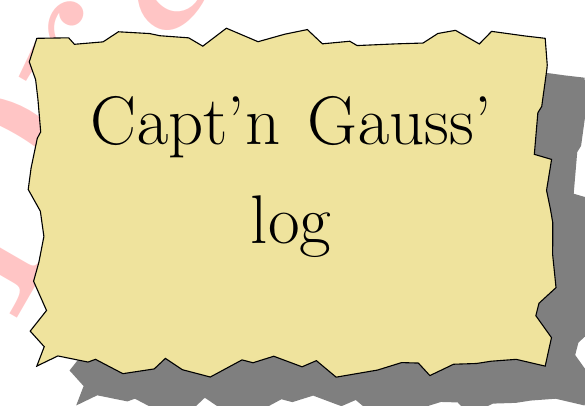
\begin{tikzpicture}[pencildraw/.style={ %%% https://tex.stackexchange.com/questions/86150/torn-page-effect/86151#86151
            decorate,
            decoration={random steps,segment length=8pt,amplitude=4pt}
          } %
        ]
        \node[preaction={fill=black,opacity=.5,transform canvas={xshift=.5cm,yshift=-.5cm}},pencildraw,draw,fill=paper,text width=.45\textwidth,inner sep=.5cm]
             {
               \vspace{-.7cm}
               \begin{center}\HUGE Capt'n \ \ Gauss' \ \  log \end{center}\vspace{.6cm} {\Huge\textit\context}
             };
  \end{tikzpicture}}
  
\end{tabular*}

\vfill



\begin{tikzpicture}
  \node[preaction={fill=white,opacity=0},inner sep=.5cm] 
             {
               \begin{minipage}{\textwidth}\Huge\example\end{minipage}
             };
  \end{tikzpicture}





\vfill


\includegraphics[width=2in]{bammLogo.png}
\hfill

\includegraphics[width=3in]{logoPirate.png}
\hfill
\raisebox{2cm}{\begin{tabular}{c}
\huge How's this math? \\
\qrcode[height=1.5in]{\mathConnections}
\end{tabular}}

}


\begin{document}

\begin{context}
  Avast, me hearties! Today I was stackin' me cups and noticed
  somethin' peculiar.
  \\[1cm]
  The number o' cups I was stackin' seemed t'
  follow a pattern. At first, I thought it was just me imagination,
  but

  the more I stacked,

  \qquad\qquad the more pattterns


  \hfill  I saw!
\end{context}

\begin{directions}
  \begin{itemize}
    \item Count how many cups are in triangular stacks that are 2, 3,
      4 (and so on) high.
    \item Look for patterns!
    \item How many cups are required for a given height?
  \end{itemize}
\end{directions}

\begin{example}

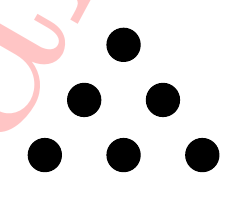
\begin{tikzpicture}
\foreach \i in {1,...,3} {
    \foreach \j in {1,...,\i} {
        \filldraw ({\j-\i/2},-\i*0.7) circle (6pt);
    }
}
\end{tikzpicture}
\hfill
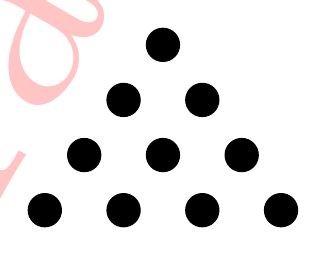
\begin{tikzpicture}
\foreach \i in {1,...,4} {
    \foreach \j in {1,...,\i} {
        \filldraw ({\j-\i/2},-\i*0.7) circle (6pt);
    }
}
\end{tikzpicture}
\hfill
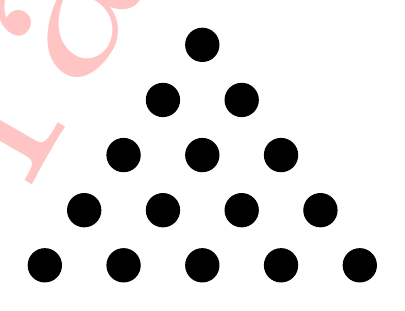
\begin{tikzpicture}
\foreach \i in {1,...,5} {
    \foreach \j in {1,...,\i} {
        \filldraw ({\j-\i/2},-\i*0.7) circle (6pt);
    }
}
\end{tikzpicture}
\hfill
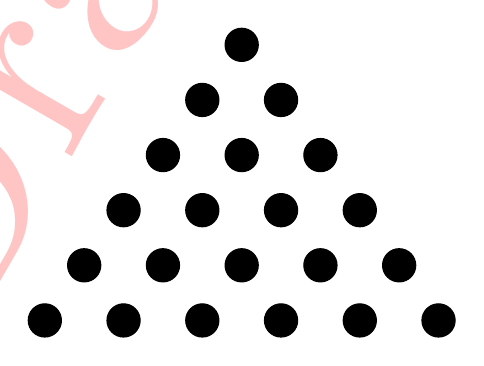
\begin{tikzpicture}
\foreach \i in {1,...,6} {
    \foreach \j in {1,...,\i} {
        \filldraw ({\j-\i/2},-\i*0.7) circle (6pt);
    }
}
\end{tikzpicture}
\end{example}

\begin{mathConnections}
  https://bartsnapp.github.io/Math-Outreach-Exhibits/cupStacking/
\end{mathConnections}
\end{document}
